\documentclass[11pt,a4paper]{article}
\usepackage[utf8]{inputenc}
\usepackage[T1]{fontenc}
\usepackage[margin=19mm]{geometry}
\usepackage{amsmath,graphicx,booktabs,array,longtable,caption}
\usepackage[hidelinks]{hyperref}
\setlength{\tabcolsep}{3pt}
\setlength{\parindent}{0pt}
\setlength{\parskip}{6pt}
\title{Upright survival and position recovery in torque limited balancing robots}
\author{Michael Agbo}
\date{12 November 2026}
\begin{document}
\maketitle
\section*{Abstract}
Remaining upright and returning to a prescribed position are different objectives for a balancing robot. We examine this distinction in a nonlinear planar wheeled inverted pendulum with motor reaction torque, input saturation, and sampled feedback. A deterministic sweep evaluates a fixed PID-type controller and a linear quadratic regulator (LQR) over 819 shared combinations of initial tilt, signed external force, and motor torque limit. The PID-type controller recovers in 215 conditions, remains upright without settling in 220, and falls in 384. LQR recovers in 357 and falls in 462. Every non-recovering PID-type survivor ends outside the position tolerance. An equilibrium calculation identifies a continuum of positions determined by the stored tilt integral. All 220 cases remain unsettled when extended from 10 to 30 seconds. A post hoc ablation that removes only the integral gain produces 433 recoveries and 386 falls, converting all 220 originally unsettled cases to recoveries while introducing two additional falls. These results demonstrate that controller ordering depends on the outcome definition and the particular implementation. They do not establish superiority of a controller class. The accompanying data, figures, and code provide a reproducible simulation analysis; matched controller tuning, measurement imperfections, payload variation, and hardware validation remain necessary extensions.

Keywords: wheeled inverted pendulum; saturation; PID-type control; linear quadratic regulation; recovery criteria; reproducible simulation

\section*{1 Introduction}
Balancing control must prevent excessive body tilt while managing wheel motion and actuator effort. A robot can satisfy the first objective yet stop away from its reference position. For inspection or manipulation, that residual translation may be operationally important even when the body is nearly vertical. A comparison based only on whether the robot falls therefore answers a different question from a comparison based on full positional recovery.

This study evaluates two fixed controllers on a transparent nonlinear model. It separates three finite-horizon outcomes: recovery to prescribed tilt, position, and speed bounds; upright survival without recovery; and crossing a declared fall threshold. The central question is how these definitions interact with torque saturation and controller structure. We report paired outcomes on identical conditions, rather than comparing favourable examples chosen separately for each controller.

The numerical study also exposes a structural feature of the chosen PID-type implementation. Integrating body tilt while feeding back position allows a nonzero stored integral to balance a nonzero position error. We derive the associated equilibrium relation and examine it through longer simulations and an integral-gain ablation. This is an analysis of the implemented controller, not a proposed new PID algorithm or a general result about all PID designs.

\section*{2 Related work and scope}
PID and LQR comparisons on self-balancing robots are established. Lau et al. [1] report hardware comparisons and a hybrid controller, including a tradeoff between tilt regulation and translational motion. Laddach et al. [2] derive PID-type settings from linear-quadratic design and validate them in simulation. These studies make a broad claim of novelty for a PID-versus-LQR comparison inappropriate. Our controllers are not reproductions of either published implementation, and their reported numerical performance is not directly comparable with ours.

More complete wheeled inverted pendulum research considers constraints, model fidelity, and physical validation. Albert et al. [3] combine constrained trajectory generation with feedback and report experiments. Measurement and communication effects are also active control problems: Music et al. [4] evaluate networked balancing with delay management. Their results motivate a separate sensing-and-delay study, but our present controller inputs are exact simulated states.

Payload adaptation is likewise an existing research direction. Baek et al. [5] estimate changes in equilibrium associated with unknown payloads and validate a physical wheeled pendulum. Song et al. [6] develop a gain-scheduled controller-observer framework for configuration and payload variation in simulation. The present robot has one fixed rigid body and no payload variation. These references delimit the current scope rather than establish a new research gap.

The contribution of this manuscript is a reproducible analysis of an explicit model and two specified gain sets: a three-way outcome map, a paired comparison, and a mechanism check for the observed positional non-recovery. The literature search was targeted rather than systematic. A claim that the evaluation protocol or equilibrium observation is novel is not made.

\section*{3 Nonlinear plant and sampled implementation}
The planar state is s = [x, v, theta, omega], where x is axle displacement from its starting point, v is horizontal velocity, theta is forward body tilt from upright, and omega is angular velocity. Positive displacement and tilt point to the right in the side view. The control torque tau is the sum of the two wheel-motor torques; the body experiences the opposite reaction torque. A horizontal disturbance force F acts at the body centre of mass.

\begin{equation}a=M+m+2I_w/r^2,\qquad b(\theta)=ml\cos\theta,\qquad d=I+ml^2\end{equation}
\begin{equation}a\ddot{x}+b(\theta)\ddot{\theta}=\tau/r-b_xv+ml\sin\theta\,\omega^2+F\end{equation}
\begin{equation}b(\theta)\ddot{x}+d\ddot{\theta}=mgl\sin\theta-\tau-b_\theta\omega+Fl\cos\theta\end{equation}
Here M denotes translating base mass, m the body mass, l its centre-of-mass distance from the axle, I its inertia about that centre, Iw the inertia of each wheel, and r the wheel radius. The mass matrix includes the rotational inertia of both wheels. The disturbance enters both translation and body rotation. Linear drag coefficients bx and btheta act on v and omega. The coupled equations follow from rigid-body kinetic and potential energy with ideal rolling and the stated generalized forces.

\textbf{Table 1 Nominal physical and numerical parameters}
\begin{longtable}{p{0.477\linewidth}p{0.198\linewidth}p{0.225\linewidth}}
\toprule
Quantity & Value & Unit \\ \midrule \endhead
Translating base mass M & 0.35 & kg \\
Body mass m & 1.20 & kg \\
Axle to body centre l & 0.18 & m \\
Body centre inertia I & 0.012 & kg m\textsuperscript{2} \\
Each wheel inertia Iw & 0.00012 & kg m\textsuperscript{2} \\
Wheel radius r & 0.045 & m \\
Gravity g & 9.81 & m/s\textsuperscript{2} \\
Translation drag bx & 0.08 & N s/m \\
Rotation drag btheta & 0.002 & N m s/rad \\
Control interval & 0.005 & s \\
Nominal torque limit & 0.70 & N m \\
Declared fall angle & 45 & deg \\
\bottomrule
\end{longtable}
The parameters in Table 1 are illustrative and have not been identified from hardware. The model excludes yaw, wheel slip, finite traction, electrical motor dynamics, impacts, sensor errors, and delay. It imposes no bound on horizontal travel. These assumptions permit controlled numerical experiments but prevent direct interpretation as a robot safety envelope.

The controller is evaluated every 5 ms and its saturated command is held during the interval. The plant is integrated with fourth-order Runge-Kutta (RK4). The baseline uses one physics step per control interval. A fall is detected at a control-step endpoint when the absolute tilt reaches 45 degrees; motion after that event is not simulated. A second JavaScript implementation supports interactive replay. Numerical tests compare that implementation against the Python reference.

\section*{4 Controllers and equilibrium mechanism}
The PID-type controller combines proportional and derivative tilt feedback, an integral of tilt, and proportional position and velocity feedback. It receives the same full simulated state as LQR; it is not a single-loop tilt-only PID. The implemented unsaturated command is

\begin{equation}\tau_{\rm raw}=14\theta+2\omega+2x+3v+0.4z\end{equation}
The integral state z starts at zero. At each sample, a candidate z + theta times the sample interval is clipped to plus or minus 0.25 rad s. It is accepted if the resulting raw command is within the torque limit or if command and tilt have opposite signs, allowing the integral to unwind. The final torque is clipped to the stated symmetric motor limit. Gains were selected by manual nominal-trial adjustment before the large sweep; no matched tuning budget or held-out tuning set was used.

LQR is designed from a centred finite-difference linearization about the upright zero state. The state cost is Q = diag(12, 2, 120, 2) and the scalar input cost is R = 1 in the stated SI coordinates. Solving the continuous algebraic Riccati equation gives the following state-feedback law, before applying the same torque saturation.

\begin{equation}\tau_{\rm raw}=-Ks,\qquad K=[-3.46410,\,-4.06357,\,-15.96706,\,-2.35048]\end{equation}
The continuous linear closed-loop poles have negative real parts. A separate zero-order-hold calculation verifies local sampled-data stability at the 5 ms control interval. Neither calculation certifies global recovery under saturation. Q and R encode this particular local design preference; changing the torque limit does not redesign the gains.

At a stationary, unforced upright equilibrium, the plant equations require zero torque. The PID-type law then admits the relation below. Thus a nonzero integral state can support a nonzero position even with zero tilt and velocity.

\begin{equation}x_*=-\frac{k_i}{k_x}z_*=-0.2z_*\end{equation}
Within the integral-state clamp, this family permits offsets up to 0.05 m in magnitude. The recovery test uses a tighter 0.03 m position bound. In the unsaturated augmented linear model, the poles are approximately -223.053, -7.835, -0.9896 plus or minus 0.6560i, and zero. The zero mode is consistent with a family of equilibria rather than asymptotic convergence to one specified position. This local argument explains a possible residual offset; it does not establish the global basin of any equilibrium or predict all saturated transients.

\section*{5 Experimental protocol}
The baseline Cartesian grid contains nine initial tilts from -20 to 20 degrees in 5-degree increments, thirteen force values from -30 to 30 N in 5 N increments, and seven total torque limits: 0.1, 0.2, 0.3, 0.4, 0.5, 0.7, and 1.0 N m. Each controller therefore encounters 819 shared conditions, yielding 1,638 baseline trials. Initial position and velocities are zero. A nonzero force pulse acts from 2.0 to 2.2 s; zero-force conditions receive no pulse. Each simulation stops at 10 s or at the first declared fall.

Recovery requires the final trajectory to remain within 1 degree of upright, 0.03 m of the initial position, and 0.03 m/s speed for at least one second. Recovery time is measured from the end of the force pulse; for zero-force trials it is measured from time zero. It is the first sampled time after the final threshold violation, provided at least one second remains. A robot that does not fall but does not meet this definition is labelled upright but unsettled. The term recovery here is a finite-horizon operational criterion, not a proof of asymptotic stability.

Metrics include peak absolute tilt, maximum absolute displacement, recovery time, squared-torque integral, and time spent in command saturation. Squared-torque integral is a control-effort proxy, not energy consumption. Falls before the scheduled push are recorded separately. Recovery-time comparisons use only conditions where both controllers recover; the denominator and resulting selection are stated explicitly.

Three additional analyses were designed after inspecting the baseline outcomes. First, all 220 upright but unsettled PID-type cases are continued with unchanged settings to 30 s. Second, only the PID integral gain is set to zero and the full 819-condition grid is repeated without retuning the remaining gains. Third, the position tolerance is varied from 1 to 6 cm while retaining the other recovery bounds and final one-second window. These are exploratory mechanism and sensitivity analyses, not preregistered confirmatory experiments.

The original 1,638 trial metrics were reproduced exactly at their stored precision before further analysis. All 705 grid cells adjacent to an outcome change along at least one of the three axes were subsequently re-evaluated with two RK4 physics substeps per control interval. The controller, force timing, and fall-detection interval remained at 200 Hz. This extends the original 32-cell audit and distinguishes integration refinement from a change in controller sampling.

The parameter grid is deterministic and deliberately constructed. Counts and paired differences are descriptive properties of these evaluated conditions. We do not treat grid cells as independent random samples from a deployment population, perform significance tests, or attach binomial confidence intervals. Reported maps resolve sampled transitions and do not certify behaviour between grid points.

\section*{6 Results}
\textbf{Table 2 Baseline outcomes on identical conditions}
\begin{longtable}{p{0.252\linewidth}p{0.162\linewidth}p{0.162\linewidth}p{0.162\linewidth}p{0.162\linewidth}}
\toprule
Controller & Recovered & Unsettled & Fallen & Total \\ \midrule \endhead
PID-type & 215 & 220 & 384 & 819 \\
LQR & 357 & 0 & 462 & 819 \\
\bottomrule
\end{longtable}
Table 2 distinguishes upright survival from positional recovery. PID-type survives in 435 conditions, compared with 357 for LQR, but only 215 PID-type trials satisfy the full recovery criterion. Consequently, the apparent ordering reverses when the endpoint changes from survival to recovery. Figure 1 shows the distribution across torque limits, and Figure 2 shows selected outcome maps. The full atlas is supplied in the technical report.

\begin{figure}[htbp]
\centering
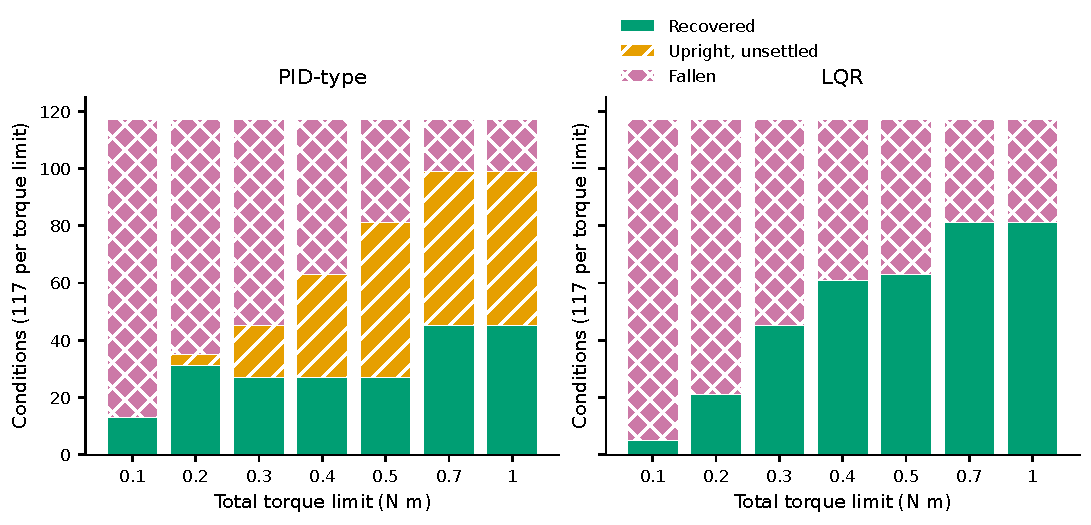
\includegraphics[width=\linewidth,height=.65\textheight,keepaspectratio]{../../figures/fig01_outcomes_by_torque.pdf}
\caption{Outcome counts at each torque limit. Each bar contains 117 conditions: nine initial tilts and thirteen signed pushes. Colours and hatching distinguish recovery, upright non-recovery, and fall. All other model and gain settings are fixed.}
\end{figure}
\begin{figure}[htbp]
\centering
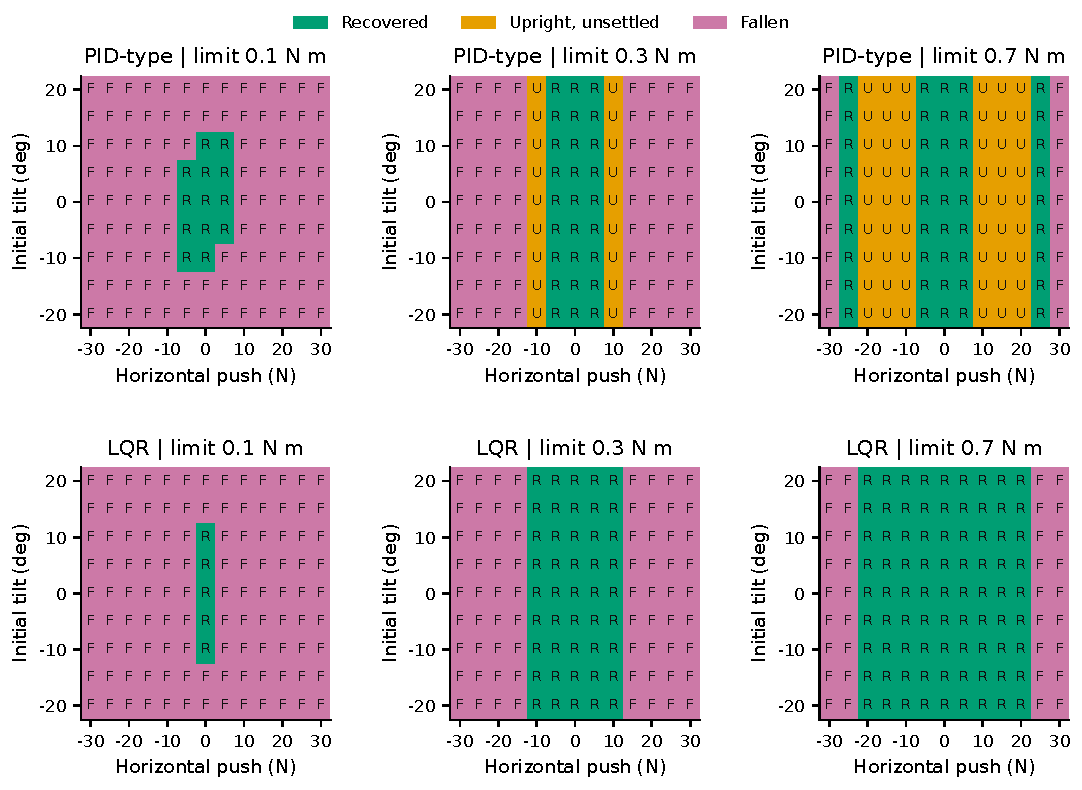
\includegraphics[width=\linewidth,height=.65\textheight,keepaspectratio]{../../figures/fig02_selected_failure_maps.pdf}
\caption{Sampled outcome maps for three torque limits. R denotes recovered, U upright but unsettled, and F fallen. The cells show evaluated points; boundaries between colours are not certified continuous operating limits. Complete maps for all seven limits appear in the technical report.}
\end{figure}
The paired outcomes in Figure 3 provide a stronger description than marginal totals. Both controllers fall in 384 shared conditions and recover in 161. There are 54 conditions where PID-type recovers and LQR falls, and 24 where PID-type remains upright but unsettled while LQR falls. In 196 other conditions, LQR recovers while PID-type remains unsettled. No sampled condition has a PID-type fall and LQR survival. Before the scheduled nonzero push, PID-type has already fallen in 48 trials and LQR in 72; those failures cannot be attributed to exposure to the full planned pulse.

\begin{figure}[htbp]
\centering
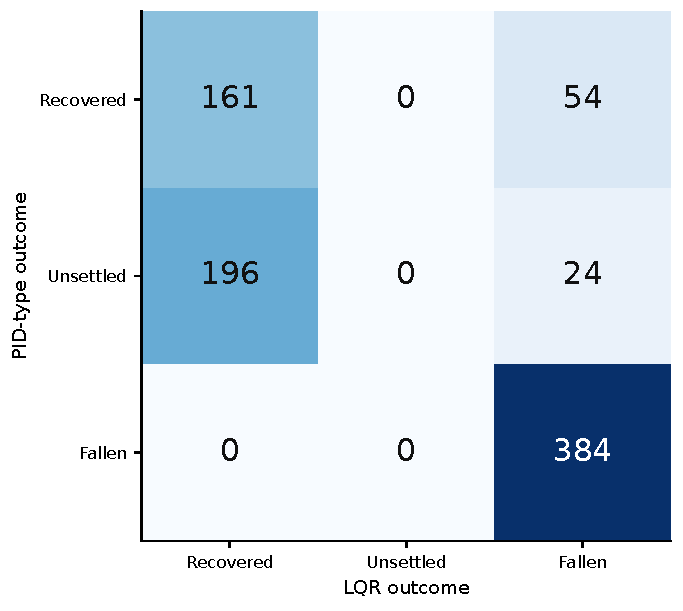
\includegraphics[width=\linewidth,height=.65\textheight,keepaspectratio]{../../figures/fig03_paired_outcomes.pdf}
\caption{Paired outcomes across the same 819 physical conditions. Rows are PID-type outcomes and columns are LQR outcomes. Off-diagonal entries reveal disagreements that marginal success counts conceal.}
\end{figure}
Among the 161 jointly recovering conditions, median recovery times are 4.080 s for PID-type and 3.055 s for LQR. The median paired difference, LQR minus PID-type, is -0.990 s; it is not the difference between the marginal medians. Median maximum displacements are 0.334 m and 0.300 m respectively. Median squared-torque integrals are 0.010854 and 0.011967 (N m)\textsuperscript{2} s. Thus faster recovery in this matched subset does not coincide with a lower median torque-effort proxy. Figure 4 shows individual paired observations rather than hiding the tradeoff in one aggregate score.

\begin{figure}[htbp]
\centering
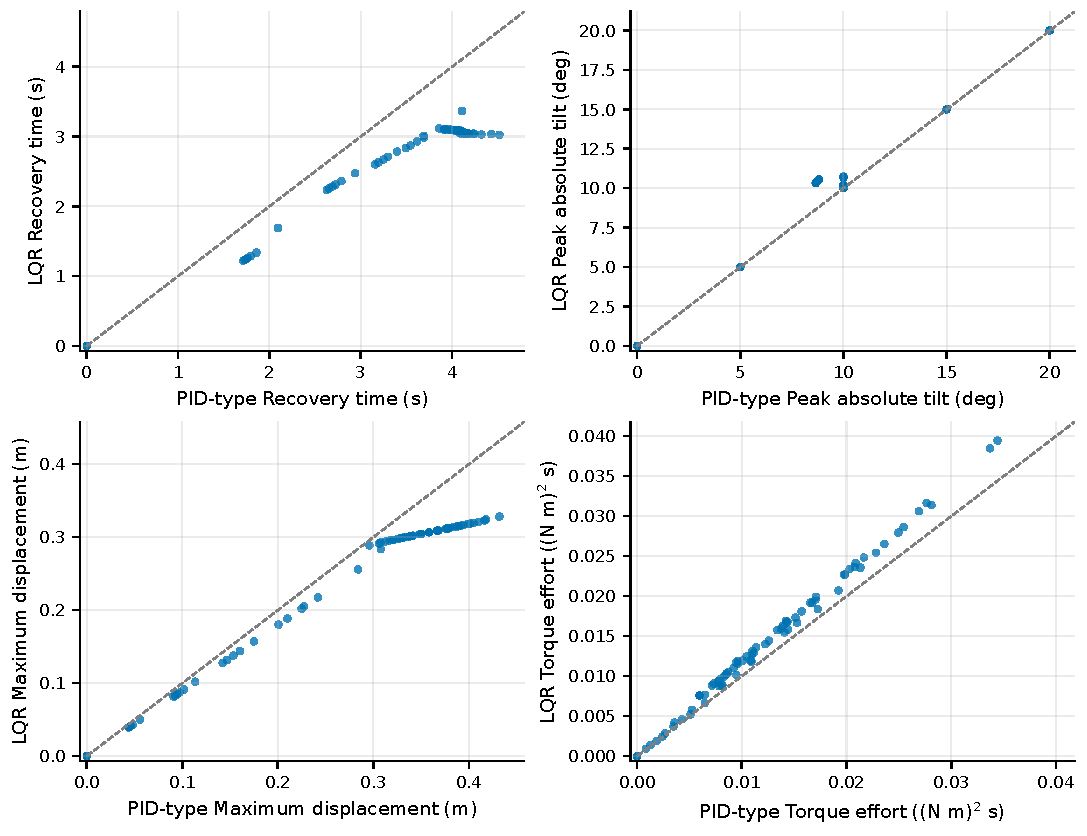
\includegraphics[width=\linewidth,height=.65\textheight,keepaspectratio]{../../figures/fig04_matched_recovery_metrics.pdf}
\caption{Paired metrics restricted to the 161 conditions in which both controllers recovered. Points below the dashed identity line have a lower LQR value. This matched subset excludes every fall and non-recovery and must not be interpreted as an unconditional controller ranking.}
\end{figure}
Figure 5 illustrates a nominal recovering condition and a condition that exposes the PID-type offset. Both trajectories are selected for explanation after the sweep. They are not used as evidence that one controller is generally superior. The force pulse, position tolerance, tilt tolerance, and torque bounds are shown explicitly so that transient response can be distinguished from terminal positional error.

\begin{figure}[htbp]
\centering
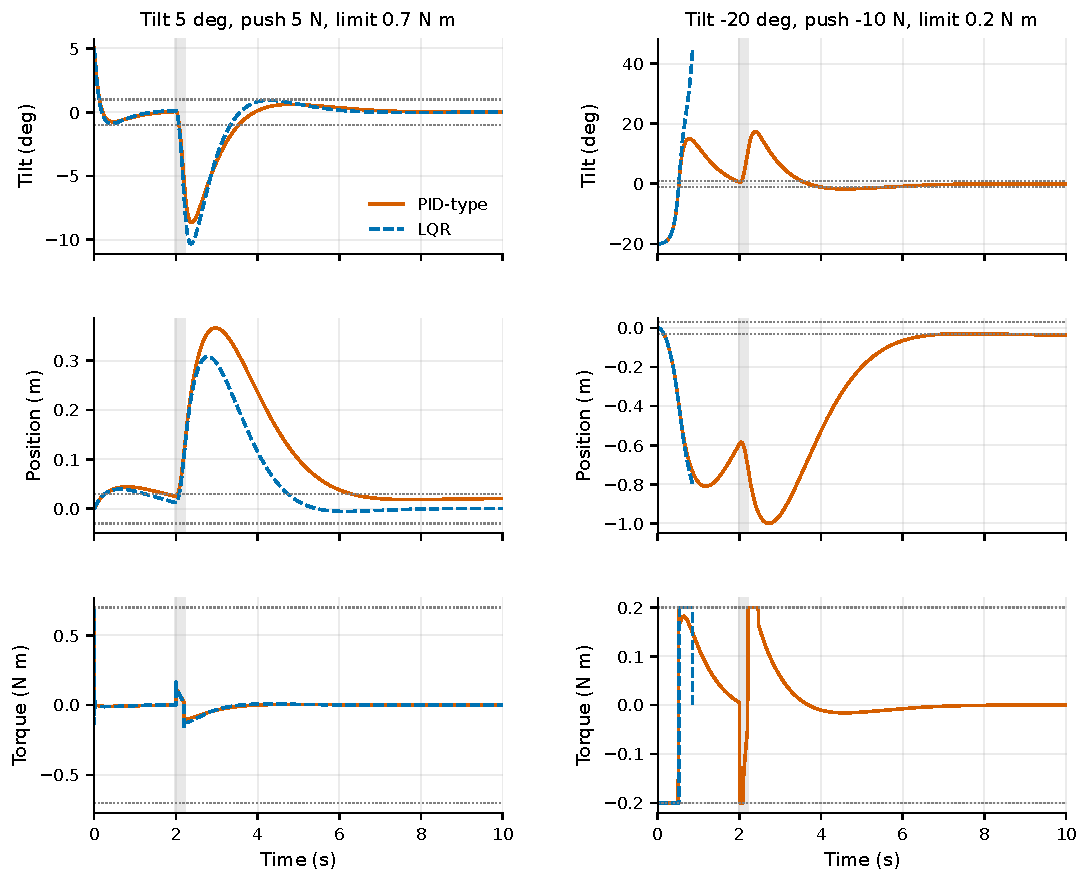
\includegraphics[width=\linewidth,height=.65\textheight,keepaspectratio]{../../figures/fig05_response_trajectories.pdf}
\caption{Illustrative trajectories for a nominal recovering condition (left) and the first PID-type unsettled condition in the original sweep order (right). Grey bands mark the force pulse. Dotted lines show the tilt and position recovery tolerances and the motor torque limits. These post hoc examples are explanatory, not representative statistical samples.}
\end{figure}
All 220 upright but unsettled PID-type trials end beyond the 3 cm position tolerance; their absolute final positions range from 3.0713 to 4.1306 cm. None has a final tilt error larger than 1 degree. Extending each case to 30 s produces no recoveries and no falls: all 220 remain unsettled. At 30 s, the largest absolute difference between the simulated position and the integral-dependent equilibrium prediction is below 2.8 \ensuremath{\times} 10\textasciicircum{}-12 m. That small number is an internal numerical-consistency result, not a statement about physical modelling accuracy. Figure 6 shows the predicted equilibrium and the persistent position distribution.

\begin{figure}[htbp]
\centering
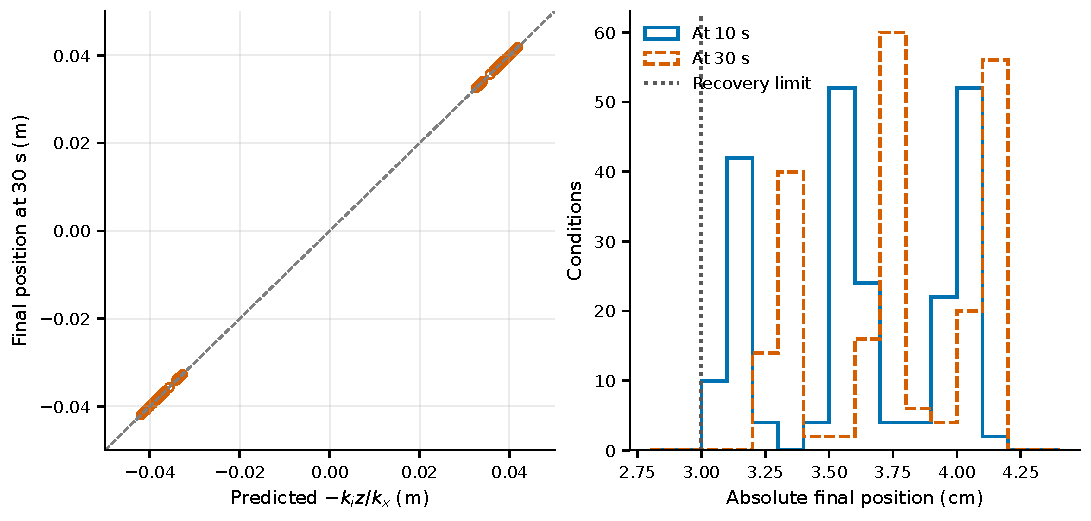
\includegraphics[width=\linewidth,height=.65\textheight,keepaspectratio]{../../figures/fig06_integral_equilibrium.pdf}
\caption{Post hoc extension of all 220 originally unsettled PID-type trials to 30 s. Left: the measured position is compared with the equilibrium relation x = -(ki/kx) z. Right: the final-position distributions at 10 and 30 s relative to the 3 cm recovery limit. No controller gains or physical parameters change.}
\end{figure}
Removing only the integral gain produces 433 recoveries, zero upright unsettled trials, and 386 falls. All 220 originally unsettled trials recover under the ablated controller. Of the 215 original recoveries, 213 remain recoveries and two become falls. The original 384 falls remain falls. Figure 7 therefore supports a specific mechanism: the stored tilt integral explains the persistent offsets in these trials, while its removal slightly changes the saturated transient failure set. The ablation is not evidence that integral action is generally undesirable.

\begin{figure}[htbp]
\centering
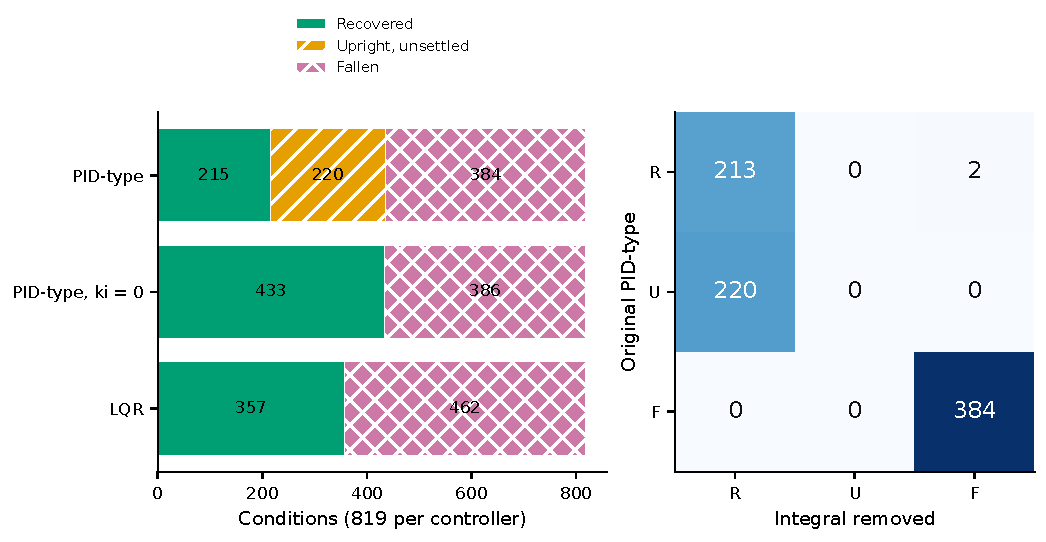
\includegraphics[width=\linewidth,height=.65\textheight,keepaspectratio]{../../figures/fig07_integral_ablation.pdf}
\caption{Post hoc integral ablation on the full original grid. Only ki is changed from 0.4 to zero; all other PID-type gains, model parameters and limits remain fixed. The right matrix pairs original and ablated outcomes (R recovered, U unsettled, F fallen). This isolates an implementation choice and is not a newly optimized controller comparison.}
\end{figure}
Outcome definitions materially affect the reported result. At a 1 cm position tolerance, only 61 baseline PID-type conditions count as recovered. At 4 cm the count is 381, and at 5 cm all 435 surviving PID-type conditions meet the recovery criterion. LQR retains 357 recoveries over the tested 1-6 cm tolerance range. Figure 8 demonstrates why tolerance selection must be motivated by the intended task rather than adjusted to favour a controller after seeing the outcomes.

\begin{figure}[htbp]
\centering
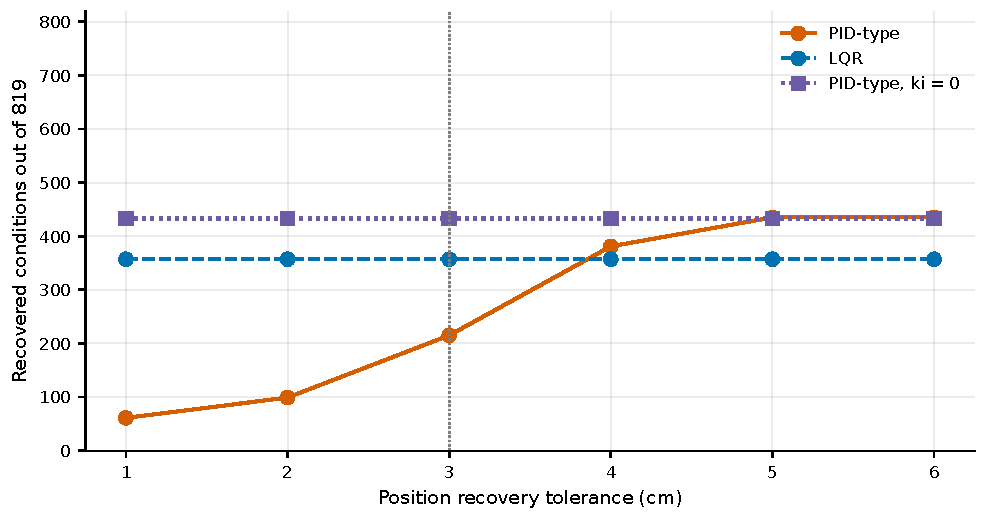
\includegraphics[width=\linewidth,height=.65\textheight,keepaspectratio]{../../figures/fig08_tolerance_sensitivity.pdf}
\caption{Post hoc sensitivity of the recovery label to the position tolerance. The final one-second dwell, 1 degree tilt bound, 0.03 m/s speed bound and 10-second horizon remain fixed. The dotted vertical line marks the original 3 cm tolerance. Curves are deterministic grid counts, without probability or confidence-interval interpretation.}
\end{figure}
The extended integration audit found 0 outcome changes across all 705 boundary-adjacent cells when the physics step was halved. This supports the reported classifications at the tested resolution. It does not prove a continuous region of attraction, remove the finite fall-detection interval, or validate the physical parameter choices.

\section*{7 Discussion and limitations}
The results should be interpreted as a comparison of two implementations, not two controller classes. Both controllers use full exact state information, but their objectives and tuning procedures differ. The PID-type law includes an integral state absent from LQR, and the LQR weights were not selected to match a specified PID transient or effort budget. The ablation changes the aggregate ranking again. A broader claim would require a transparent tuning protocol, multiple gain sets, held-out conditions, and preferably matched performance or effort constraints.

The persistent-offset result is structurally simple but consequential for evaluation. A nearly vertical robot can be labelled successful by a tilt-only test while failing a position-regulation task. In this implementation, the failure is not merely a short simulation horizon: it remains after 30 s and follows the equilibrium relation. Changing the position tolerance changes the headline count without changing any trajectory. A useful benchmark must therefore state its operational objective before controller selection.

Several model assumptions limit external validity. Perfect rolling omits traction loss; ideal torque commands omit electrical bandwidth and battery limits; exact state feedback omits measurement noise and delay; and one fixed rigid body omits load-induced changes in mass distribution. The 45-degree threshold is an analysis convention rather than a measured contact event. Horizontal travel is unconstrained, so a controller may survive by moving farther than a real workspace permits.

The finite grid and chosen force pulse cover only a small family of disturbances. They do not include arbitrary initial velocities, changing reference positions, continuous disturbance spectra, slopes, or terrain. Signed symmetry provides coverage in both directions, but it does not create independent replications. The integrations are deterministic; physical trials would require calibrated parameters, repeated measurements, and an uncertainty model. The baseline is also exploratory rather than preregistered.

A stronger follow-on study should first separate sensor noise from observation delay, evaluate an explicit state estimator, and then introduce physically consistent payload changes. Payload mass, centre of mass, and inertia must change together. Frozen-gain robustness should be evaluated before comparing adaptation or redesign, with held-out test conditions and a defined tuning budget. Prior work on delay and payload compensation [4-6] means that a new contribution must be stated more narrowly than simply adding those features.

\section*{8 Conclusions}
For the model and gain sets studied, upright survival and position recovery give different controller orderings. The original PID-type controller survives more grid conditions, while LQR recovers in more. A stored tilt integral accounts for all 220 persistent PID-type positional non-recoveries. Removing that integral eliminates those offsets but adds two falls. The main lesson is methodological: report paired outcomes, distinguish survival from task recovery, and explain controller-specific mechanisms before making broad performance claims. The present evidence establishes a reproducible simulation finding, not a validated hardware advantage or a certified safe operating region.

\section*{Data and code availability}
The accompanying research package contains the original per-trial records, configuration and source hashes, baseline reproduction diagnostics, horizon-extension and ablation data, the extended numerical audit, figure-generation code, and editable manuscript source. The interactive local simulation can replay tested conditions. No public repository or archival identifier has yet been assigned. Reproduction instructions and software versions are supplied in the technical report and package README.

\section*{Research integrity and author review}
All reported results are numerical simulations; no hardware, human-participant, or field experiments were conducted. The analyses and writing were prepared with AI-assisted coding and drafting. The author must independently review the model, code, calculations, citations, and claims before submission and adapt any disclosure to the selected venue. Funding, affiliation, and conflict-of-interest declarations are not asserted in this version.

\section*{References}
[1] L. B. Lau, N. S. Ahmad, and P. Goh. Self-balancing robot: modeling and comparative analysis between PID and linear quadratic regulator. International Journal of Reconfigurable and Embedded Systems 12(3), 351-359, 2023. \url{https://doi.org/10.11591/ijres.v12.i3.pp351-359}\par
[2] K. Laddach, M. Czyzniewski, and R. Langowski. A selection of PID type controller settings via LQR approach for two-wheeled balancing robot. 2021 25th International Conference on Methods and Models in Automation and Robotics, 378-383, 2021. \url{https://doi.org/10.1109/MMAR49549.2021.9528471}\par
[3] K. Albert, K. S. Phogat, F. Anhalt, R. N. Banavar, D. Chatterjee, and B. Lohmann. Structure-Preserving Constrained Optimal Trajectory Planning of a Wheeled Inverted Pendulum. arXiv:1811.12819v2, 2019. Preprint version. \url{https://arxiv.org/abs/1811.12819v2}\par
[4] Z. Music, F. Molinari, S. Gallenmuller, O. Ayan, S. Zoppi, W. Kellerer, G. Carle, T. Seel, and J. Raisch. Design of a Networked Controller for a Two-Wheeled Inverted Pendulum Robot. arXiv:1812.03071v2, 2019. Preprint version; related publication DOI 10.1016/j.ifacol.2019.12.153. \url{https://arxiv.org/abs/1812.03071v2}\par
[5] D. Baek, Y. Sim, A. Purushottam, S. Gupta, and J. Ramos. Toward Control of Wheeled Humanoid Robots with Unknown Payloads: Equilibrium Point Estimation via Real-to-Sim Adaptation. arXiv:2403.10948v2, 2024. Preprint. \url{https://arxiv.org/abs/2403.10948v2}\par
[6] Y. Song, G. Wan, and X. Cao. Gain-Scheduled Control of a Wheeled Inverted-Pendulum Robot with Load-Induced Equilibrium Drift Compensation. Applied Sciences 16(10), 4876, 2026. \url{https://doi.org/10.3390/app16104876}\par
\end{document}
